\section{UI Integration}
The MARS system is already equipped with a User Interface where one can create a project, manage the different resources, run the simulation and
analyze the results. The different back end services (See \ref{table:MARS Resource Hierarchy Service Overview}) are integrated in a Graphical
User Interface so that an domain expert i.e. ecologists who are not computer experts could utilize the powerful tools that the framework offers.
The aspect that this framework is intended to be used also for user with less expertise in the technical field makes it an absolute necessity that
the functions that the archive service delivers be part of the graphical system.

\begin{figure}[H]
    \centering 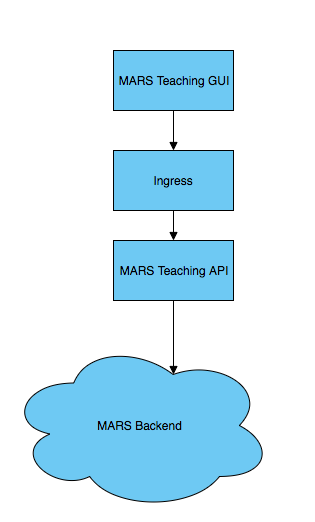
\includegraphics[scale=0.6]{grafiken/marsIngress.png}
    \caption{MARS cloud overview with the UI}
    \label{fig:marsCloudUI}
\end{figure}

Figure \ref{fig:marsCloudUI} illustrates a high level communication between UI and the back end services. It is to be noted that the backend services
are running in an self contained environment which is not available to the outside ports and other clients. Therefore, 
to make the services available the Ingress\footnote{https://kubernetes.io/docs/concepts/services-networking/ingress/} is present. Ingress contains
a set of rules which allows inbound connections to reach the services that are inside the cluster(encausplated from outside). In the MARS system
the Ingress creates a reverse proxy to the teaching API. The teaching API is the bridge between the different backend services and the GUI. The purpose
of making the requests via the Teaching API is to have a more secure system as it authenticates if the client which is making the requests is the right owner or 
is an intruder. This check is done as the teaching API provide a authentication token i.e. Bearer token to the GUI and this token has to be included in the
header of ever request made making it more secure as only the clients having the tokens can make a successful request. After a successful request to the Teaching API
it forwards the request to the concerning web service.


The first step needed for a complete integration of the Archive service for the UI is to determine which endpoints are going to be exposed to the outside ports.
The endpoints decided to be exposed for the thesis are archive project, retrieve project and get status. These endpoints must be programmatically added
in the Teaching API which is written in GO Lang. Lastly, after the endpoints are made available the UI components are added in the Teaching GUI service
written in Angular 4. 

\begin{figure}[H]
    \centering 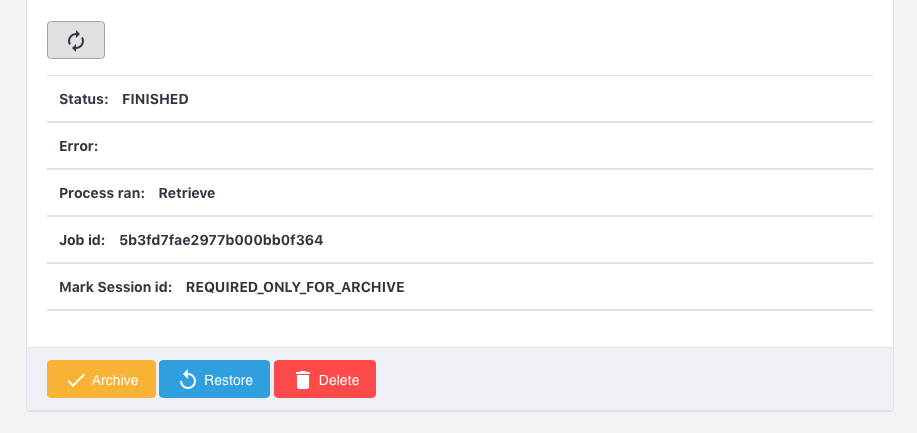
\includegraphics[scale=0.5]{grafiken/archiveUI.png}
    \caption{Archive service UI controls in the MARS Teaching UI}
    \label{fig:archiveUI}
\end{figure}

Figure \ref{fig:archiveUI} illustrates the integrated archive service in the MARS Teaching GUI where an retrieve job is being executed. The archive process
status can be seen in the same area where the retrieve information is seen after a simple refresh.
